\documentclass[conference,compsocconf]{IEEEtran}
\usepackage{amsmath,amssymb,amsfonts,float,graphicx,bm,psfrag,amsmath,amsthm}
\usepackage{algorithm, algorithmic,CJK,color,color,geometry,url}
\usepackage{graphicx,cite,bm,psfrag,amsmath}
\def\mmax{\mathop{\mbox{\scriptsize max}}}
\def\argmin{\mathop{\mbox{arg\,min}}}
\def\argmax{\mathop{\mbox{arg\,max}}}
\newcommand{\defequal}{\stackrel{\mathrm{def}}{=}}
\renewcommand{\vec}[1]{{\ensuremath{\boldsymbol{#1}}}}
\newcommand{\popt}{\ensuremath{P^{(K)}_{opt}}}
\renewcommand{\algorithmicrequire}{ \text{Input:}} %Use Input in the format of Algorithm
\renewcommand{\algorithmicensure}{ \text{Procedures:}} %UseOutput in the format of Algorithm
\newtheorem{mypro}{Proposition}
\IEEEoverridecommandlockouts
\pagestyle{plain}
\renewcommand{\algorithmicrequire}{ \textbf{Input:}} %Use Input in the format of Algorithm
\renewcommand{\algorithmicensure}{ \textbf{Procedures:}} %UseOutput in the format of Algorithm
\geometry{left=0.59in, right=0.59in, top=0.7in, bottom=0.69in}
\DeclareRobustCommand*{\IEEEauthorrefmark}[1]{%
	\raisebox{0pt}[0pt][0pt]{\textsuperscript{\footnotesize\ensuremath{#1}}}}
\def\BibTeX{{\rm B\kern-.05em{\sc i\kern-.025em b}\kern-.08em
		T\kern-.1667em\lower.7ex\hbox{E}\kern-.125emX}}
%\usepackage[colorlinks]{hyperref}
%\hypersetup{colorlinks=true,linkcolor=blue,filecolor=magenta,urlcolor=cyan}
\urlstyle{same}

%\usepackage{booktabs}
\usepackage[T1]{fontenc}
\usepackage[table]{ xcolor}
\setlength{\columnsep}{0.25in}
\begin{document}
	\title{Achieving the Highest Average User Data Rate in Wireless Network using Reinforcement Learning}
	\author{Qi Cao\IEEEauthorrefmark{1*}, Mingqi Yuan\IEEEauthorrefmark{2*}, Siliang Zeng\IEEEauthorrefmark{1}, Man-On Pun\IEEEauthorrefmark{1}\IEEEauthorrefmark{\dagger} and Yi Chen\IEEEauthorrefmark{1}\\
	\IEEEauthorrefmark{1}The Chinese University of Hong Kong, Shenzhen\\
	Guangdong, China, 518172\\
	\IEEEauthorrefmark{2}Mingqi's affiliation
	\thanks{*Authors contribute equally. \IEEEauthorrefmark{\dagger}Corresponding author, email: SimonPun@cuhk.edu.cn. This work was supported by}}
\maketitle
	
	\begin{abstract}
		The frequency resources allocation in wireless communication is aimed at improving some predefined network-level key performance indicator (KPI) such as the network capacity, the average user data rate, and the $5\%$-tile user data rate. This allocation is essentially realized by matching candidate users with resource block group (RBG) each occupying a transmission time interval and a fixed bandwidth, and this process can be referred as user scheduling. When users are with full buffers, it is known that \textit{opportunistic} scheduling is optimal in terms of achieving the highest average user date rate (AUDR). However, in the bursty buffer case, the optimal scheduling has not been revealed, especially when it is influenced by mechanisms from both physical (PHY) layer and media access control (MAC) layer. In this context, we leverage reinforcement learning (RL) to train a convolutional neural network (CNN), namely RBGNet, which is able to flexibly take dynamic number of users' states as input and produce feasible scheduling solutions leading to high AUDR. With a self-built simulator involving essential mechanisms in PHY and MAC layer, the superiority of our proposed RBGNet is verified, compared to \textit{opportunistic} and \textit{proportional fairness (PF)} scheduling. As such, this work provides a remarkable scheduling algorithm in achieving the highest AUDR in bursty buffer cases.
	\end{abstract}
	
	\begin{IEEEkeywords}
		RBG allocation, Reinforcement learning, CNN, Highest average user data rate
	\end{IEEEkeywords}
	
	\section{Introduction}
	
	User scheduling is a classical problem in wireless communications, which can be traced back decades ago \cite{borst2001dynamic}. That being said, the optimal strategy has never been found. It can be explained from two different angles which are: first the optimality is difficult to determine when it comes to the comprehensive performance of throughput, fairness and delay; and second even if the key performance indicator (KPI) is well defined, the optimality only exists in theoretical models but never a practical system involving numerous transmission mechanisms. On the other hand, the meaning of so-called user scheduling can be extended to a wide range, which is not limited to power allocation, user pairing, transmission time interval (TTI) and resource block group (RBG) arrangement.

    Among the early works, proportional fair (PF) scheduling is an essential one as it balances between throughput and fairness \cite{tse2001multiuser}. The PF scheduling is proved to maximize the sum of logarithmic average user rates $\sum \log R_i$, being $R_i$ the individual user average data rate \cite{kelly1998rate}, and its multi-carrier version is given in \cite{kim2005proportional}, forming the basic RBG allocation algorithm for today's wireless network. More recently, the PF scheduling is widely adopted or further investigated in various scenarios, for instance, the non-orthogonal multiple access system \cite{gemici2019user,saito2015system}. And it triggers gradient scheduling algorithm studies aimed to maximize a utility function named $\alpha$-fairness, which generalizes the objective of the scheduling \cite{ameigeiras2012traffic}.
    
    In this paper, we focus on the RBG allocation but as far as we know, the optimal strategy achieving the highest average user data rate is never revealed in bursty buffer cases. Even so, the optimal for full buffer cases is known as opportunist algorithm, which simply greedily allocates RBGs to the users with highest expected data rate in each TTI \cite{borst2001dynamic}. It is worth mentioning that mathematical modeling is almost impossible to solve the problem. The technical challenges come from that: first, a wireless communication network is highly complex with many components and mechanisms, rendering the whole system analytically intractable; second, it is difficult to accurately describe channel transfer function, inter-cell interference and user distribution and movement etc; finally, network events are mostly stochastic such as user arrival, traffic load and channel variations. 
	
	On the other hand over the recent years, artificial intelligence (AI), specifically machine learning, has entered many industrial fields, be it traditional or emerging, and plays the role of a mighty competitor challenging existing rules and stereotypes. The exploding demand of data over the air loads increasingly more pressure on current mobile Internet, while model-driven solutions are leading us to the bottleneck. In such a context, the combination of machine learning and wireless communications is an essential and promising next step, where there are already studies trying the methodology in power allocation \cite{sun2018learning,sato2019approximation} and modulation and coding rate selection \cite{bruno2014robust}.
	
	In this paper, we attempt to leverage deep reinforcement learning to allocate network-level performance using both MAC and PHY layer information. Our main contributions are as follows:
	\begin{itemize}
		\item In a sophisticated wireless network simulator, we collect the feasible  features and define the framework of our proposed deep reinforcement algorithm. Even though the long-term objective is achieving the highest average user data rate, it is not clear what should the reward be according to an action. As such, we developed a deviation based reward function which is shown to be effective in achieving our objective.
		\item The number of users attached on a base station (BS) is always dynamic. To facilitate the practical implementation of our proposed RBGNet. We construct a flexible CNN configuration, which could cope with dynamic number of users and arrange them to fixed number of RBGs. Besides, a training algorithm accordingly is developed to contribute the convergence and efficacy of the RBGNet.
		\item With a large number of various discrete/continuous counters and complicated operating mechanisms such as Out Loop Link Adaptation (OLLA) and Hybrid Automatic Repeat reQuest (HARQ) and retransmission in wireless communication network, we demonstrate that using the proposed RBGNet is possible to outperform traditional PF or opportunist scheduling in terms of average user data rate.
	\end{itemize}
	

	
	In what follows, we introduce the task specifications and dataset establishment in Sec. II and the designed DNN configuration is detailed in Sec. III. The proposed training algorithm is elaborated in Sec. IV. Finally Sec. V presents the simulation results before conclusion is given in Sec. VI.
	
\section{Simulator Basics}


This section introduces the details of the built simulator which follows the protocol of LTE \cite{protocol2013}. Specifically,  $K$ RBGs share a frequency bandwidth $B$ to serve Poisson-arriving downlink users with expected arrival rate $\lambda$. The base station is equipped with two transmit/receive antennas respectively while UEs are equipped with one transmit antenna and two receive antennas. The transmit power is beyond the scope of this paper and so assumed to be the same to all users. The LTE protocol allows a user to suggest an appropriate MCS via feeding back a channel quality indicator (CQI), which eventually stabilizes the block error rate (BLER) of the user to a certain level. The simulator randomly generates an ACK/NACK message by a probability to every transmission, indicating its successful/unsuccessful delivery. The probability is related to the MCS chosen and the actual signal-to-noise (SNR) ratio and an offset per user. In what follows, some critical mechanisms are elaborated, from which it can be seen that building mathematical models to derive a user scheduling in any sense of optimality is intractable.

%Being under bursty buffer traffic, the system randomly initializes the buffer size between $0.5$~Kbytes and $3$~Mbytes for each arrived UE. In addition, the noise power density is at $-174$~dBm/Hz, and the transmit power of each RB is fixed at $18$~dBm. In what follows, 

\subsubsection{Out Loop Link Adaptation}
On the user side, a CQI level representing an SNR interval is periodically computed and reported. Thus the received instantaneous SNR directly influences the selection of MCS. %It is known that neither aggressive (high) or conservative MCS selection is inappropriate. Higher MCS level implies bigger transmission block (TB) size but also higher BLER, and vice versa. The most appropriate MCS as to have the highest expectation of the amount of data that can be successfully transmitted is in line with a BLER level of 90\%. 
However it should be noted that there is an offset reflecting the detection sensitivity which is a natural property per user and unknown to the BS. Thus, to compensate the discrepancy between the chosen MCS and the optimal MCS for different users. An OLLA process occurred on BS to carry out to offset a CQI value $q$ is used and given by
\begin{equation}
\bar{q}=\left[q+\alpha\right],
\end{equation}
being $[\cdot]$, the rounding operation and $\bar{q}$ the offset CQI readily for MCS selection. Note that $\alpha$ is the adjustment coefficient updated every time an ACK/NACK message is captured, i.e.

\begin{equation}
\alpha=
\begin{cases}
\alpha+s_A, & \mathfrak{A} = 1, \\
\alpha+s_N, & \mathfrak{A} = 0,
\end{cases}
\end{equation}
being $\mathfrak{A}=1$ the ACK message and $\mathfrak{A}=0$ the NACK message being 1 for ACK and 0 for NACK. The update rate $s_A$ being positive and $s_N$ being negative can be customized, and it is trivial to show that the final BLER converges to $-s_N/s_A$.

\subsubsection{Transmission Block Formation}
Due to the relationship among CQI, MCS and spectral efficiency (SE) is fixed. Assume $\mathcal{M}(\bar{q})$ denotes the mapping from the offset CQI $\bar{q}$ to its SE, then, the estimated data rate of UE $n$ in RBG $k$ can be obtained by
\begin{equation}
R_{n,k}=\sum_{\ell\in \mathcal{G}(k)} B\mathcal{M}(\bar{q}_{n,\ell}),
\end{equation}
where $\mathcal{G}(k)$ is the set of all RBs in RBG $k$, and $\ell$ is the index of an RB, and $\bar{q}_{n,\ell}$ is the offset CQI level of UE $n$ in RB $\ell$. The BS adopts a default MCS when the CQI is not given, which especially happens at the beginning of a transmission. 

When multiple RBGs are allocated to the a UE, they are utilized to convey one data packet (Transport Block, TB) with the same MCS. That is to say, even though the estimated data rate $R_{n,k}$ is adopted in the user scheduling, but the size of the TB loading on the RBG might differ. Suppose $\{\bar{q}_{n,\ell}\}$ with size $L$ is the set of all RBs allocated to UE $n$, then the actual TB size is written as
\begin{equation}
T_n=LB\mathcal{M}\left(\bigg\lfloor\frac{1}{L}\sum_{\ell}\bar{q}_{n,\ell}\bigg\rfloor\right),
\end{equation}
where $\lfloor\cdot\rfloor$ is the floor function. However if a UE fails to acquire any RB, $T_n$ will be equal to zero at the current TTI.

%as a consequence, the moving average throughput will goes down and the priority of the UE in all RBG will increase.


\subsubsection{Hybrid Automatic Repeat reQuest and Retransmission}
\begin{figure}
	\centering
	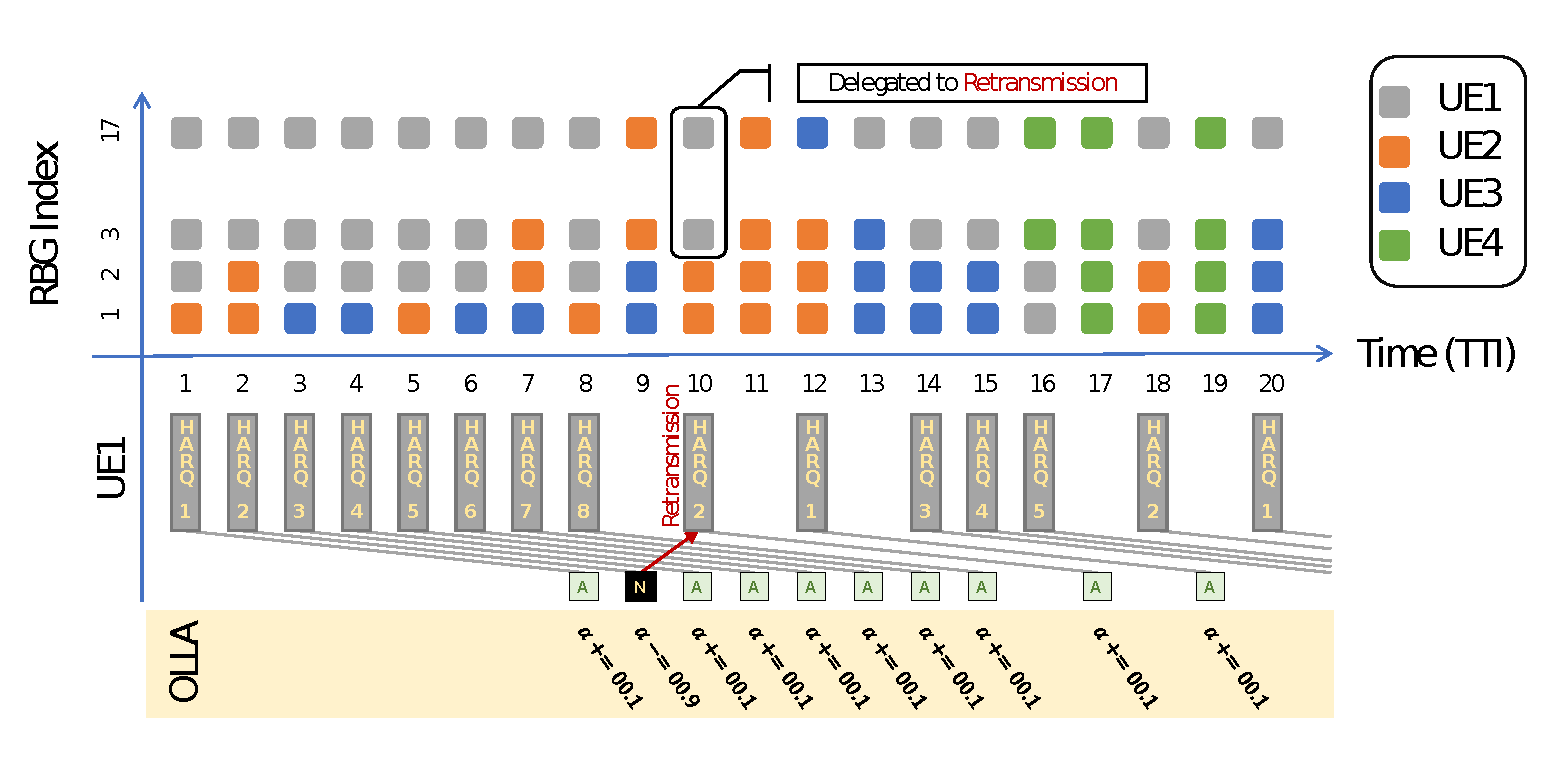
\includegraphics[width=1\linewidth]{Figs/system.eps}
	\caption{Network Mechanisms}
	\label{sys}
\end{figure}

When the TB is set for a UE, the corresponding data will be loaded to the HARQ buffer and held there until being dropped as an outcome of either successful transmission or expiration. The convenience for the mechanism is that whenever a retransmission is required, the data can be directly fetched in HARQ buffer. The BS prepares eight HARQ processes for each UE. The BS will see an ACK/NACK message from the corresponding user in seven TTIs. In the case of ACK, the HARQ process terminates, while in the case of NACK, a retransmission is triggered. The RBGs initially delegated to the first transmission will conduct the retransmission, thus being unavailable for user scheduling. The MCS selection and TB size remains the same for the retransmission and the HARQ process will expire at five times of consecutively failure, which literally causes the so-called packet loss.


\section{Objective}
Assume a user $n$ arrives at TTI $t_{n,a}$, and the service is completed at TTI $t_{n,t}$. We have the user data rate equal to
\begin{equation}
C_n=\frac{S_n}{t_{n,t}-t_{n,a}}.
\end{equation}
However, as some users may not finish transmitting all data in the buffer at the moment of compute the data rate, thus we could alternatively use the following temporal user data rate written as
\begin{equation}
\bar{C}_n[t]=\frac{\sum_{i=t_{n,a}}^{t}T_{n}[i]\mathfrak{A}_n[i]}{\min(t,t_{n,t})-t_{n,a}}, \quad t>t_{n,a}.
\end{equation}
Note that $\bar{C}_n[t]$ has no meaning when $t\leq t_{n,a}$. Our objective in this paper is to find an effective user scheduling maximizing the expectation of all arrival users, i.e.

$$\max\lim_{t\rightarrow\infty}\mathbb{E}\{\bar{C}_n[t]\}, \quad\forall n.$$
In the sequel, we sometimes omit the TTI index for brevity.
%\section{Proposed Reinforcement Learning Solution}
%
%\subsection{Environment and Agent}
%
%\subsection{RBGNet Configuration}
%
%\subsection{Training Method}

\section{Framework of Reinforcement Learning}
A reinforcement learning system consists of two essential components i.e. an interactive environment and an agent. With respect to our RBG allocation, the scheduling process is discrete owing to its intrinsic motivation.
Thus the trajectory of interaction can be viewed as a sequence of state-action-reward tuples $
\{s_t, a_t, r_t\}$. In what follows, the architecture of our reinforcement learning system is elaborated in detail.
\subsection{Interaction environment}
The environment gives the agent according feedbacks including the status of the next state and rewards for the current actions. For a complex system as wireless communication network, the construction of states is challenging and crucial.
\subsubsection{State}
In terms of RBG allocation, the state of environment is composed of status of all users in the base station. That is to say, every attribute should constitute a part of state, including the known and the unknown. However as the agent is planted on the BS, reasonable and quantitative attributes feasible on the BS side are carefully selected and gathered in table \ref{tb:1}.


\begin{table}[H]
	\caption{Attributes of state}\label{tb:1}
	\centering
	\begin{tabular}{lcc}
		\hline
		Attr.                    & Layer   & Dim.       \\ \hline
		RSRP                    & PHY & 1         \\
		buffer size             & MAC & 1         \\
		historical throughput        & MAC & 1         \\
		Olla offset             & MAC & 1         \\
		scheduled times         & MAC & 1         \\
		RB CQI                  & PHY & Num. of RB \\
		average of RB CQI       & PHY & 1         \\
		std. of RB CQI          & PHY & 1         \\ \hline
	\end{tabular}
\end{table}

%Thus the dimension of state for each user is $d_s=num_{RB}+7$
The construction of the subsequent deep neural network is also related to the specific dimension of the state.


\begin{figure*}[htp]
	\centering
	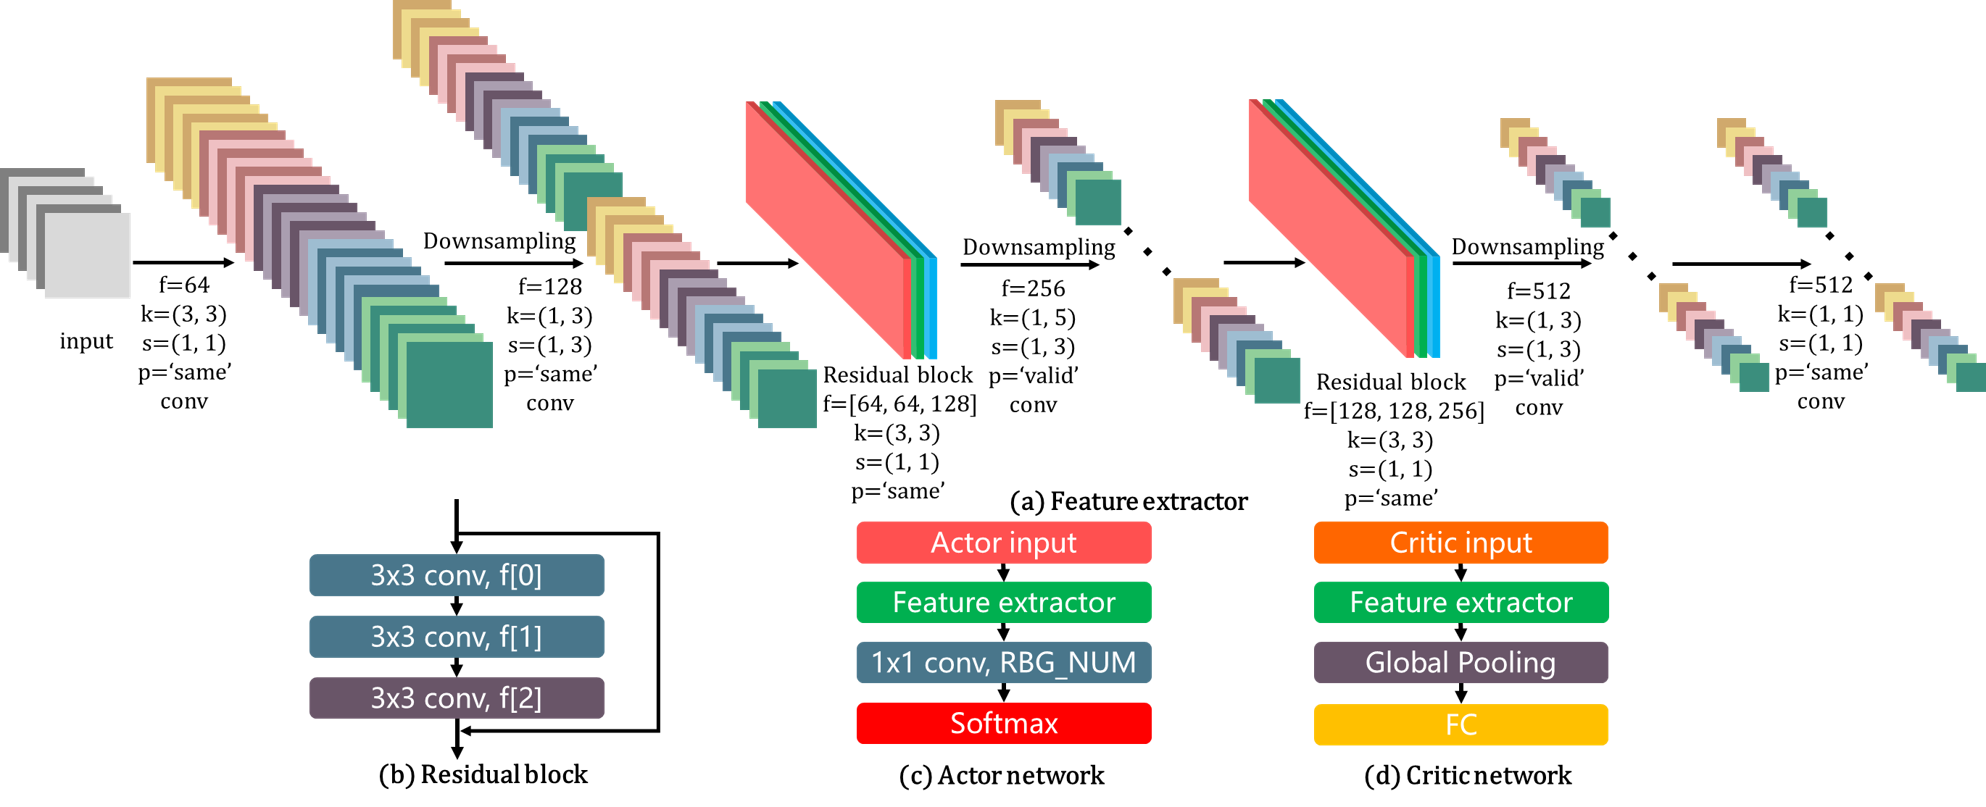
\includegraphics[scale=0.4]{Figs/RBGNet.eps}
	\caption{Architecture of RBGNet.The parameters of downsampling layers were configured skillfully based on $ d_{feature} $}\label{fig:arch}
\end{figure*}
\subsubsection{Reward}
The reward signal characterize the optimization target, which motivates the agent to explore any possible solutions. As the system is aimed to maximize the AUDR, the configuration of reward function must take transmission rate into consideration. From the point of view of a user $n$, the optimistic data rate regardless of the outcome of ACK/NACK in TTI $t+1$ can be written as

\begin{equation}
\begin{aligned}
\hat{C}_n[t]&=\frac{\bar{C}_n[t-1]*(t-1-t_{n,a})+R_n[t]}{t-t_{n,a}}\\
&=\bar{C}_n[t-1]\frac{t-1-t_{n,a}}{t-t_{n,a}}+\frac{R_n[t]}{t-t_{n,a}}\\
&=const.+\Delta r_n[t]
\end{aligned}
\end{equation}
where the first term is irrelevant to any actions but the second term is fully controllable. We define the second term as the \textit{data rate deviation} $\Delta r_n[t]=R_n[t]/(t-t_{n,a})$, Thus we design the reward function as
\begin{equation}
r_t = \log_{\eta} \left(\sum_{i=1}^{N}\Delta r_i[t]+1\right),
\end{equation}
where the $\log$ function and $\eta$ are introduced to ensure that the reward function is strictly incremental and locally bounded, since it is conceived that the boundedness of reward function promotes the convergence of the model during training.

\subsection{Agent}
In this section, we elaborates the agent who takes actions on observations of the environment. In details, the optimization algorithm and network design are elaborated the sequel.
\subsubsection{Deep Deterministic Policy Gradient}
The optimization algorithm gives the method of exploration and adjustment. A \textit{Deep Deterministic Policy Gradient} algorithm which is model-free, off-policy actor-critic algorithm uses deep function approximators that can learn policies in high-dimensional, continuous action spaces
\cite{Lillicrap2015Continuous}. The whole algorithm requires two important roles, namely an actor and a critic. The actor network takes actions and the critic network estimates the reward, so let $ \mu (s|\mathbf{\Theta}^{\mu})$ denote the actor and $ Q (s,a|\mathbf{\Theta}^{Q})$ the critic respectively. Yet,
the application of DDPG for RBG allocation is illustrated in the Algorithm \ref{al:1}.

\begin{algorithm}
	\caption{DDPG for RBG Allocation}
	\begin{algorithmic}[1]\label{al:1}
		\STATE \textbf{Initialization:} Randomly initialize the weights in actor and critic network $ \mathbf{\Theta}^Q $ and $\mathbf{\Theta}^{\mu}$;  Set a replay buffer $B$ and learning rate $\tau$.
		%\STATE Initialize target network $ Q^\prime $ and $ \mu^\prime $ with weights $ \mathbf{\Theta}^{Q^\prime} \leftarrow \mathbf{\Theta}^Q $, $ \mathbf{\Theta}^{\mu^\prime} \leftarrow \mathbf{\Theta}^{\mu}$ 
		
		\FOR{Epoch$ =1:M$}
		\STATE Randomly Generate $K$ users.
		%\STATE Receive initial observation state $ s_1 $ 
		\FOR{$t=1:T$}
		\STATE Add users to base station according to Poisson distribution.
		\STATE Execute action $ a_{t}=\mu (s_t|\mathbf{\Theta}^{\mu}) $ and observe new state $ s_{t+1} $.
		\STATE Receive reward $ r_{t} $ and store the transitions $ (s_{t}, a_{t}, r_{t}, s_{t+1}) $ in $ B $.
		\STATE Sample a random minibatch of $ N $ transitions $ (s_i, a_i, r_i, s_{i+1}) $ from $ B $.
		\STATE Set $ y_i = r_i + \gamma Q^{\prime}(s_{i+1}, \mu^{\prime}(s_{i+1}|\mathbf{\Theta}^{\mu^{\prime}})|\mathbf{\Theta}^{Q^{\prime}}) $
		\STATE Update critic by minimizing the loss function: \\$ L=\frac{1}{N} \sum_{i}(y_i - Q(s_i, a_i|\mathbf{\Theta}_Q)^2)$
		\STATE Update the actor policy using the sampled gradient:
		$$
		\begin{aligned}
		&\nabla_{\mathbf{\Theta}^{\mu}}\mu|_{s_i}\approx \\ &\frac{1}{N}\sum_i \nabla_{a}Q(s, a|\mathbf{\Theta}^Q)|_{s=s_i,a=\mu(s_i)}\nabla_{\mathbf{\Theta}^{\mu}}\mu(s|\mathbf{\Theta}^{\mu})|_{s_i}
		\end{aligned}
		$$
		\STATE Update the target networks:
		$$
		\mathbf{\Theta}^{Q \prime} \leftarrow \tau\mathbf{\Theta}^{Q} + (1-\tau)\mathbf{\Theta}^{Q \prime}
		$$
		$$
		\mathbf{\Theta}^{\mu \prime} \leftarrow \tau\mathbf{\Theta}^{\mu} + (1-\tau)\mathbf{\Theta}^{\mu \prime}
		$$
		\ENDFOR
		\ENDFOR
	\end{algorithmic}
\end{algorithm}


The DDPG is designed for continuous action space, whereas the RBG allocation is a discrete action. To make the discrete task become continuous will contribute to the model convergence.

\subsubsection{RBGNet}
In the real communication process, the number of users in the base station changes frequently, which means that the state observed by the agent is not always of the same dimension, causing great challenges to the network design of the actor and critic network. For instance, conventional fully-connected neural network is excluded for the limitation of its fixed input and output. To address this problem, CNN is considered helpful in building the two components, which can accept scalable input when the network is fully convolutional \cite{long2015fully}. We name this network structure by \textit{RBGNet}.

\subsubsection{Backbone}
Figure \ref{fig:arch} illustrates the architecture of proposed RBGNet. The actor and critic take the same feature extractor to handle the input, which can effectively simplify the design of architecture and facilitate the convergence of network parameters. Besides, to avoid the vanishing gradient problem, two residual block is inserted \cite{He2016Deep}. Also, we mean to design such a very deep network for more representative power to handle the complex scheduling problem. 

\textbf{Remark:}
For the actor network, the input's shape is $( d_s, K, 1)
$
where $ K $ is the quantity of user, $ 1 $ is regarded as channel of image processing.
Apply downsampling to the input for three times, the shape of output map is: 
$
d_{output \, map}=(batch \, size, K, 1, F) 
$
where $ F $ is the quantity of filters in the last convolution layer of feature extractor.
As shown above, the third dimension of $ d_{output \, map} $ is $ 1 $, which is necessary for the subsequent process, 
so the parameters of downsampling layer should be configured skillfully based on the $ d_s $.

Then, this map is submitted to the output layer, which is a convolution layer with (1, 1) filters and Softmax activation function, and 
the Softmax score characterizes the allocation result.
Specially, the quantity of filters in the output layer is equal to the quantity of RBG, which aims to make each RGB be allocated by
an independent filter.
Based on the configuration, each RBG was allocated independently but the prediction is still joint.
The final result has nothing to do with the $ d_s $ but only related to the quantity of users and RBG.
$$
d_{softmax \, score}=(batch \, size, K, 1, Num_{RBG})
$$

For the critic network, the input is the integration of state and action, thus the input's shape is 
$$ 
d_{critic \, input}=(batch \, size, d_s+Num_{RBG}, K, 1) 
$$
Firstly, the input is submitted to feature extractor to produce intermediate feature.
Secondly this map is processed by the Global Pooling layer, which can replace the fully connected layer to accept scalable input. \cite{Lin2013Network}
Thus the output is only related to the quantity of filters in the last convolution layer of feature extractor.
$$
d_{output \, map}=(batch \, size, F) 
$$
Finally, this map is received by a fully connected layer to predict the reward.

\subsubsection{Training strategy}
The training of reinforcement learning is a difficult and long-time job.
In the early stage of the experiment, two models were established to solve the problem of full buffer case and bursty case respectively.

\begin{algorithm}
	\caption{Training strategy}
	\begin{algorithmic}[1]
		\STATE \textbf{Step 1: full buffer case training}
		\STATE
		Initialize agent $\mathcal{A}_{RL}$ and $\mathcal{A}_{Oppo}$ respectively.
		\STATE  
		Initialize $p(\mathcal{A}_{RL}) \leftarrow 0, p(\mathcal{A}_{Oppo}) \leftarrow 0$, where $ p() $ is the performance of agent, threshold $ \varphi_{1} $.
		\WHILE{$ p(\mathcal{A}_{Oppo}) - p(\mathcal{A}_{RL}) > \varphi_{1} $}
		\FOR{Epoch=1, M}
		\STATE Two agents interact with the environment to generate available experience $ E_{RL}^1$ and $E_{Oppo}^1$.
		\STATE Update $ \mathcal{A}_{RL} $ with \textbf{Mixed Experience} composed of $ E_{RL}^1$ and $E_{Oppo}^1$.
		\ENDFOR
		\STATE Update $p(\mathcal{A}^{\prime}_{RL})$ and $p(\mathcal{A}^{\prime}_{Oppo})$:
		$
		p(\mathcal{A}_{RL}) \leftarrow p(\mathcal{A}^{\prime}_{RL}), p(\mathcal{A}_{Oppo}) \leftarrow p(\mathcal{A}^{\prime}_{Oppo})
		$
		\IF{$p(\mathcal{A}^{\prime}_{RL}) > p(\mathcal{A}_{RL})$}
		\STATE Update $\mathcal{A}_{RL}$: $ \mathcal{A}_{RL} \leftarrow \mathcal{A}^{\prime}_{RL} $
		\ELSE
		\STATE continue
		\ENDIF
		\ENDWHILE
		\STATE Save the best agent model $ \mathcal{A}^{*}_{RL} $
		\STATE \textbf{Step 2: bursty case training}
		\STATE
		Initialize agent:$\mathcal{A}_{RL} \leftarrow \mathcal{A}^{*}_{RL}$
		\STATE
		Initialize $p(\mathcal{A}_{RL}) \leftarrow 0, p(\mathcal{A}_{Oppo}) \leftarrow 0$, threshold $ \varphi_{2} $
		\WHILE{$ p(\mathcal{A}_{RL}) - p(\mathcal{A}_{Oppo}) < \varphi_{2} $}
		\FOR{Epoch=1, M}
		\STATE Two agents interact with the environment to generate available experience $ E_{RL}^2$ and $E_{Oppo}^2$.
		\STATE Update $ \mathcal{A}_{RL} $ with $ E_{RL}^2$.
		\STATE Update $p(\mathcal{A}^{\prime}_{RL})$ and $p(\mathcal{A}^{\prime}_{Oppo})$:
		$
		p(\mathcal{A}_{RL}) \leftarrow p(\mathcal{A}^{\prime}_{RL}), p(\mathcal{A}_{Oppo}) \leftarrow p(\mathcal{A}^{\prime}_{Oppo})
		$
		\ENDFOR
		\IF{$p(\mathcal{A}^{\prime}_{RL}) > p(\mathcal{A}_{RL})$}
		\STATE Update $\mathcal{A}_{RL}$: $ \mathcal{A}_{RL} \leftarrow \mathcal{A}^{\prime}_{RL} $
		\ELSE
		\STATE continue
		\ENDIF
		\ENDWHILE
	\end{algorithmic}
\end{algorithm}

For bursty case, the agent can explore any possible solutions to maximize the average transmission rate since the optimal solutions is uncertain, 
and the performance of the agent successfully surpasses the \textit{Opportunistic Schedule} after lots of training.

For full buffer case, the agent was hoped to achieve the effect close to that method, 
but we've found it's difficult to achieve that only by the agent's own exploration.
\textit{Opportunistic Schedule} is a fixed method, 
so it's difficult and impractical for a network with millions of parameters to learn a fixed method by trial-and-error.
Howerver, it's clear that the \textit{Opportunistic Schedule} is the optimal solution to maximize average rate, 
which provides the best experience to guide the agent.
Therefore, the \textbf{Mixed Experience} was introduced to train the agent, which is composed of the experience both from self-exploration and \textit{Opportunistic Schedule}.
With lots of training and \textit{fine-tuning} \cite{HowardUniversal}, the agent successfully simulated the \textit{Opportunistic Schedule}.

In order to make the model compatible with both full buffer case and bursty case, a step-by-step training strategy was introduced to address this problem.
First of all, the agent is trained with \textbf{Mixed Experience} in full buffer case, which can simulate the behavior of \textit{Opportunistic Schedule}.
At this stage, the \textit{fine-tuning} operation should be repeated again and again to get the best performance.

Secondly, using bursty case to train the previous model with low learning rate.Now, the experience is not mixed, which is only from the self-exploration.
In a word, the training strategy is full of technique which should be configuration based on the specific situation.

\section{Numerical Results}




\subsection{Beach Mark Schemes}
\subsubsection{Opportunistic User Scheduling} As the optimal scheduling in terms of systematic throughput maximization, opportunistic user scheduling is quite straightforward, which can be expressed as

\begin{equation}
P^*(k)=\arg\mathop{\max}_{n}R_{n,k}.
\end{equation} 
It means each RBG selects the user suggesting the highest estimated data rate, which also implies the optimal scheduling in achieving the highest AUDR in full buffer case.


\subsubsection{Propotional Fairness User Scheduling}
To balance the system throughput and fairness, a user scheduling called proportional fairness is proposed in \cite{tse2001multiuser}, where the scheduling is achieved by allocate RBGs to different UEs. Any UE with a non-empty buffer on the BS side is a candidate to each RBG, and each RBG independently sort all UEs according to their PF values. Denote the PF value of UE $n$ on RBG $k$ within transmission time interval (TTI) $i$ by $\beta_{n,k}[i]$ computed as
\begin{equation}
\beta_{n,k}[i]=\frac{R_{n,k}[i]}{\bar{T}_n[i]},
\label{eq1}
\end{equation}
where $\bar{T}_n[i]$ is the UE's moving average historical throughput which can be expressed as
\begin{equation}
\bar{T_n}[i]=\left(1-\gamma\right)\bar{T}_n[i-1]+\gamma T_n[i-1].
\label{eq:2}
\end{equation}
In Eq. (\ref{eq:2}), $\gamma$ is the moving average coefficient, which is usually very small, and $T_n[i-1]$ is the actual TB size of UE $n$ in TTI $i-1$ interpreted as how many number of bits is sent in last TTI. We sometimes omit the TTI index for brevity in the sequel. The UEs with higher PF value are with higher priorities to capture the RBG, and the PF value of a UE to different RBGs can be different. Specifically, the PF scheduling can be expressed as
\begin{equation}
P^*(k)=\arg\mathop{\max}_{n}\beta_{n,k},
\end{equation} 
%To avoid allocate more RBGs to a UE than it needs, each RBG $k$ finds its highest PF value among all UEs $\mathop{\max}_{n}\left\{\beta_{n,k}\right\}$, and the RBG allocation is done one by one according to the ordered set in descending fashion $\left\{\mathop{\max}_{n}\left\{\beta_{n,k}\right\}\right\}$. Each time when an RBG is allocated to a UE, say $n^*$, the system checks if $n^*$ obtained enough RBG to convey all its buffer data. If so, $n^*$ will be removed from remaining RBGs' lists, which always happens when the buffer of UE $n^*$ is about to be emptied.


\subsection{Performance Comparison}
In the following, the simulator sets 50 RBs and 17 RBGs using a frequency bandwidth of $10$~MHz. The noise power density is at $-174$~dBm/Hz, and the transmit power of each RB is fixed at $18$~dBm. All performances of RL is based on a well-trained RBGNet. For both full buffer and bursty buffer cases, 100 simulations are realized and all performance data are collected independently.

The table \ref{tb:2} shows the out-performance statistics among the three user schedulings. The number in each cell indicates the percentage that the former scheduling outperforms the latter one. As expected, the opportunist scheduling beats RL and PF all in full buffer in terms of AUDR, and PF scheduling beats the rest in terms of 5\%-tile, which testifies the validity of our simulation. We highlight that in bursty buffer, our proposed RBGNet has won 96\% simulation against PF and 97\% simulations against opportunistic scheduling.

\renewcommand\arraystretch{1.5}
\begin{table}[H]
	\caption{Outperformance Comparison} \label{tb:2}
	\centering
	\begin{tabular}{c|c|c|c|c}
		\hline
		\textbf{}           & \multicolumn{2}{c|}{\textbf{Full buffer case}} & \multicolumn{2}{c}{\textbf{Bursty buffer case}} \\ \hline
		\textbf{}           & \textbf{AUDR}      & \textbf{5\%-tile}      & \textbf{AUDR}    & \textbf{5\%-tile}   \\ \hline
		\textbf{RL vs PF}   & 96\%         & 0\%                    & \textbf{96\%}                & 29\%                \\ \hline
		\textbf{RL vs Oppo} & 0\%                   & 1\%                    & \textbf{97\%}       & 79\%                \\ \hline
		\textbf{PF vs Oppo} & 0\%                   & 100\%         & 66\%                & 82\%      \\ \hline
	\end{tabular}
\end{table}


The performance gain distribution is illustrated in Fig.\ref{fig:3}, where the blue line is with reference to opportunist scheduling and the red line is with reference to the PF scheduling. The performance discussed here is AUDR only. As can be seen from the figure, even though opportunistic scheduling outperforms RL in all 100 simulation in full buffer, the RL scheduling can still provide satisfactory solutions. The worst scenario only shows a 20\% shy to the optimal, whereas actually the mean value of the AUDR degradation is 8.71\% compared to the optimal. Nevertheless, in the bursty buffer case, the RL scheduling manifest a strong superiority against other scheduling, respectively achieving a 12.17\% and 13.17\% AUDR gain compared to opportunist and PF scheduling.
\begin{figure}
	\centering
	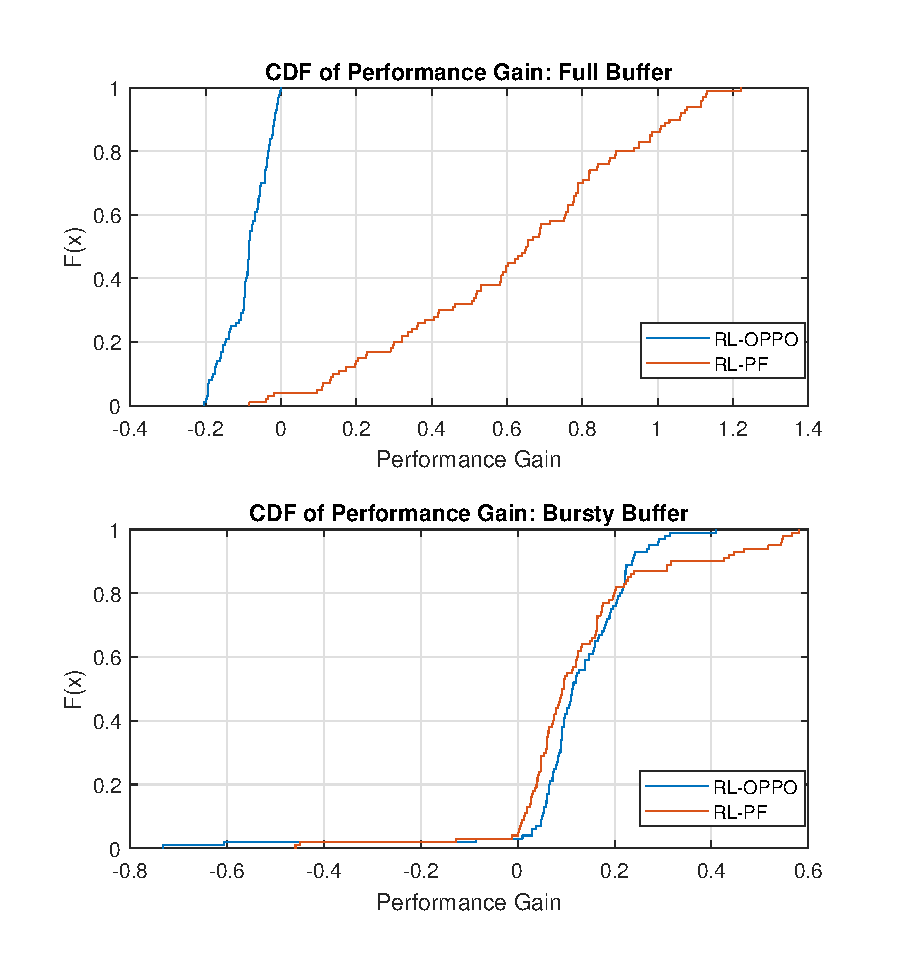
\includegraphics[width=\linewidth]{Figs/cdf.eps}
	\caption{CDF of Performance Gain}
	\label{fig:3}
\end{figure}
\section{Conclusion}

In this paper, a model-free RL user scheduling algorithm is developed to pursue the highest AUDR, where the optimal scheduling is never derived in bursty buffer case. In other words, the practical user scheduling aiming at AUDR is still a blank area. We then demonstrated the feature collection, derived a reward function and introduced the configuration of proposed RBGNet. Using our DDPG training algorithm, the RBGNet successfully converges and demonstrates outstanding performance with about 13\%  AUDR gain in contrast with existing schedulings.


\bibliographystyle{ieeetr}
\bibliography{reference}
\end{document}


